\documentclass{article}
\usepackage{graphicx}
\usepackage{amsmath}
\usepackage{algorithm}
\usepackage{algpseudocode}
\usepackage{amsfonts}

\title{Dynamic Shuffled Keyboard Stream Cipher for Encryption}
\author{Andrew R. Garcia\\garcia.gtr@gmail.com}
\date{}

\begin{document}

\maketitle

\begin{abstract}
The algorithm presented in this paper, \texttt{STREAMDICE}, is a novel stream cipher that provides encryption by considering the specific identity of characters and their relative location in the message string. \texttt{STREAMDICE} utilizes dynamically shuffled keyboards, generated by a cryptographically secure pseudo-random number generator (CSPRNG), with each keyboard shifted for every encrypted character. These shuffled keyboards are stored in memory using securely derived seeds, dependent on the provided encryption keys. This approach optimizes auxiliary space complexity while enhancing resistance to brute force attacks. The decryption process reverses the encryption protocol using the same keys.
\end{abstract}

\section{Introduction}
Effective encryption is crucial for protecting data and private information. Proper encryption ensures that unauthorized access to data is meaningless without the correct encryption keys. The algorithm presented here, \texttt{STREAMDICE}, is a stream cipher that encrypts characters (i.e., letters, numbers, and some allowed signs) by their specific identity and their relative location in the message string thread. \texttt{STREAMDICE} uses dynamically shuffled keyboards generated by a cryptographically secure pseudo-random number generator (CSPRNG), with each keyboard shifted for every encrypted character. This method obfuscates periodicity and enhances resistance to brute force attacks, making it a robust encryption solution.

\section{Related Work}
Stream ciphers like RC4, ChaCha20, and Snow 3G are widely used, employing Linear Feedback Shift Registers (LFSRs) or similar mechanisms to generate keystreams. Modern approaches focus on lightweight designs for IoT, GPU implementations for high-speed encryption, and hybrid methods combining chaos theory and stream ciphers for enhanced security and performance. \texttt{STREAMDICE} introduces a novel method by using dynamically shuffled keyboards, providing a new layer of randomness and complexity.

\section{Method}

\subsection{Unwarped Map Creation}
The unwarped map represents the original arrangement of characters on a QWERTY keyboard, including uppercase and lowercase letters, numbers, and special characters. Let \( \mathbb{C} \) be the character set used for encryption. The bidirectional map, \( p_U \), associates each character \( \mathcal{C}_i \in \mathbb{C} \)  with its corresponding index \( i \):

\begin{align}
    p_U = \{ (\mathcal{C}_i, i) \, | \, \forall i \, (\mathcal{C}_i \in \mathbb{C}) \}
\end{align}

and its inverse:

\begin{align}
    p_U^{-1} = \{ (i, \mathcal{C}_i) \, | \, \forall i \, (i \in \mathbb{N}) \}
\end{align}

\begin{figure}[h]
  \centering
  \includegraphics[width=0.7\linewidth]{img/qwerty.png}
  \caption{Standard QWERTY keyboard}
  \label{fig:keyboard}
\end{figure}

\subsection{Map Warping}
The map warping operation \( p_W \) is initialized with a \( \text{CSPRNG}(\mu_i) \) seeding, where \( \mu_i \) is a seed generated by the encryption key provided by the user. This operation reshuffles the keys, adding a layer of randomness to the encryption process. Every map warping operation produces a unique keyboard set (Figure \ref{fig:hash}).

\begin{figure}[h]
  \centering
  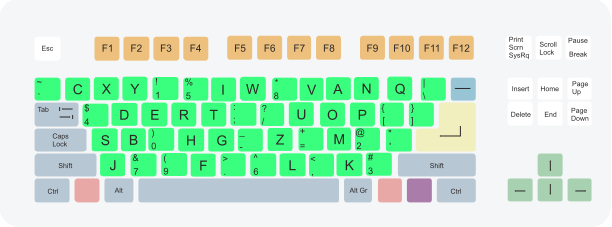
\includegraphics[width=0.7\linewidth]{img/qwerty_shuffled.png}
  \caption{Randomly-shuffled keyboard with $\mu_i$ seed \#5443}
  \label{fig:hash}
\end{figure}

\subsection{Character Encryption and Decryption Process}
The encryption process transforms input characters $\mathcal{S}_i$ into their corresponding encrypted characters $\mathcal{C}_i$ using \( p_W \) map warping. Decryption reverses this process using \( p_U \) map unwarping. For each character \( \mathcal{S}_i \) in a message string $\mathbb{S}$, the algorithm retrieves the corresponding index using \( p_U(\mathcal{S}_i) \) and applies \( p_W \) to obtain $\mathcal{C}_i$. If \( \mathcal{S}_i \) is a space, it is directly printed.

Thus, for encryption:
\begin{align}
  \forall \mathcal{S}_i \in \mathbb{S}: \quad \mathcal{C}_i = p_W(p_U(\mathcal{S}_i))
\end{align}$\mathcal{S}_i$
\begin{algorithm}
\caption{\texttt{STREAMDICE} Encryption Algorithm}
\begin{algorithmic}[1]
\State \textbf{Input:} Message string $\mathbb{S}$, Key1 $\mathrm{k_A}$, Key2 $\mathrm{k_B}$, Flag $encrypt$
\State $\text{sequence} \gets \text{Extract digits from } \mathrm{k_B}$
\State $\mu \gets \text{Compute seeds from } \mathrm{k_A} \text{ and } \mathrm{k_B}$
\For{each character $\mathcal{S}_i$ in $\mathbb{S}$}
    \If{$encrypt$}
        \State $\mathcal{C}_i \gets p_W(p_U(\mathcal{S}_i))$
    \Else
        \State $\mathcal{S}_i \gets p_U^{-1}(p_W^{-1}(C_i))$
    \EndIf
    \State Update $i \gets (i + 1) \mod \text{length}(\text{sequence})$
\EndFor
\State \textbf{Output:} Encrypted/Decrypted Message String
\end{algorithmic}
\end{algorithm}

The specific seeds are computed directly from the keys provided by the user for encryption. An $\mu$ vector contains all the $\mu_i$ seeds used to generate the shuffled keyboards. The number of $\mu_i$ seeds is equal to the number of digits provided for $\mathrm{k_B}$, computed as follows:
\[
  \mu_i = \mathrm{k_A}  + (\mathrm{k_B} // 10^{i}) \% 10
\]

\begin{figure}[h]
  \centering
  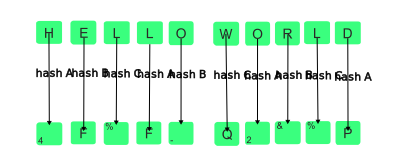
\includegraphics[width=0.7\linewidth]{img/helloworld.png}
  \caption{Encrypting \textit{hello world} with a periodically-repeating stream of 3 shuffled keyboards.}
  \label{fig:helloworld}
\end{figure}

The seeds used to generate the new keyboard, rather than the specific keyboard arrangement, are kept in memory throughout the encryption. Decryption uses the same keys to reverse the protocol, optimizing auxiliary space complexity, $\mathcal{O}(N)$, rather than encryption time complexity, $\mathcal{O}(|\mathbb{S}||\mathbb{C}|)$, where $N$ is the number of digits of $\mathrm{k_B}$.
% , while $|\mathbb{S}|$ and $|\mathbb{C}|$ are the message string length and number of keyboard characters to encrypt, respectively.

\section{Security Analysis}
\texttt{STREAMDICE} leverages cryptographically secure PRNGs and strong key derivation functions to generate seeds, ensuring robustness against brute force and cryptographic attacks. The dynamic shuffling of keyboards for each character encryption introduces high entropy, obfuscating periodicity and enhancing security.

\section{Conclusion}
\texttt{STREAMDICE} introduces a novel approach to stream ciphers by employing dynamically shuffled keyboards and secure seed management. This method optimizes memory usage while providing robust security against brute force attacks. Future work will focus on formal security proofs and performance optimizations.

\end{document}
